%% This is emulateapj reformatting of the AASTEX sample document
%%
\documentclass{emulateapj}
\usepackage[colorlinks,urlcolor=blue,citecolor=blue,linkcolor=blue]{hyperref} 
\usepackage{graphicx,natbib}
\citestyle{aa}
\usepackage[space]{grffile}
\usepackage{latexsym}
\usepackage{amsfonts,amsmath,amssymb}
\usepackage{url}
\usepackage[utf8]{inputenc}
\usepackage{fancyref}
\usepackage{hyperref}
\usepackage{multirow}
\hypersetup{colorlinks=false,pdfborder={0 0 0},}

\DeclareMathOperator{\erfinv}{erfinv}

%% You can insert a short comment on the title page using the command below.
%\slugcomment{To appear in The Astrophysical Journal (ApJ)}

\begin{document}

\title{FRB 121102: Radio Bursts Seen by Very Large Array and Implications for Overall FRB Population}
\shorttitle{FRB 121102: VLA Burst Properties}
\shortauthors{Law et al.}

\author{Casey J. Law\altaffilmark{1}}
\author{et al.}
\altaffiltext{1}{Dept of Astronomy and Radio Astronomy Lab, Univ. of California, Berkeley, CA}

\begin{abstract}
The highly-dispersed, millisecond radio transients known as Fast Radio Bursts have recently emerged as a new class...
The discovery of repeating bursts from FRB121102 has shown that at least some FRBs are not cataclysmic and opened potential for studying a homogenous sample of bursts...
Our recent coordinated campaign with the Very Large Array and Arecibo Observatory has made the first direct, arcsecond-scale localization of an FRB and unambiguously associated it with counterparts in other observations. This campaign detected nine bursts at the VLA from 2.5 to 3.5~GHz and many more at Arecibo near 1.4~GHz. The coordination of these observations allow us to refine our picture of the physical processes in FRB121102. 
With so many bursts, we can make the first reliable measures of burst flux distribution and temporal statistics...
The connection of FRB121102 to the overall population...

\end{abstract}

\section{Introduction}

The discovery of Fast Radio Bursts, a new class of millisecond-duration, highly-dispersed radio transients, has opened a whole new playground in astrophysics. 

- Physical processes

- Utility as probes

- Repeater as anomalous FRB

- VLA data provides new insight on role of repeater in overall FRB population

\section{Observations}

All observations in August and Septmeber were searched in quasi real-time by a prototype version of \emph{realfast}. \emph{realfast} is a real-time, fast imaging transient search system. The current, prototype runs on existing hardware of the VLA correlator backend, while the future \emph{realfast} will run on a dedicated GPU cluster.

Burst detections and localizations were made within hours of data being recorded.

\section{Results}

\subsection{Spectra}

\begin{figure}[htb]
\begin{center}
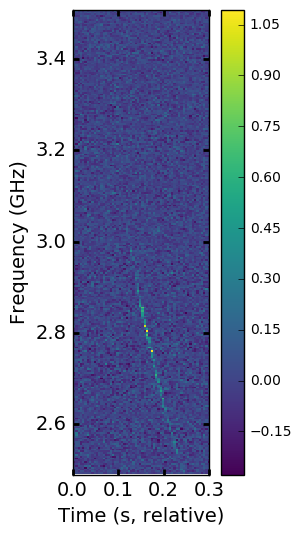
\includegraphics[width=0.3\columnwidth]{sgram_57623.png}
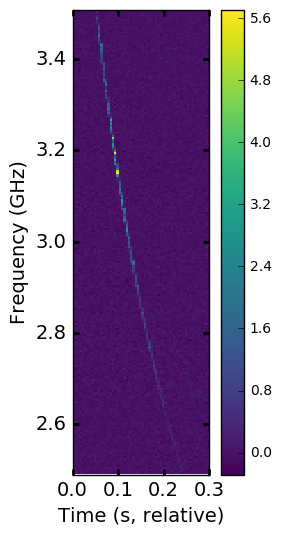
\includegraphics[width=0.3\columnwidth]{sgram_57633_scan7.png}
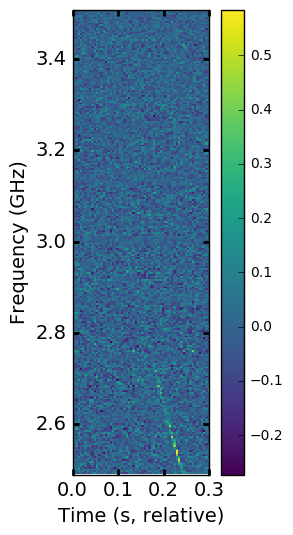
\includegraphics[width=0.3\columnwidth]{sgram_57633_scan13.png}
\caption{
\label{fig:name}}
\end{center}
\end{figure}


\subsection{Circular Polarization}


\subsection{Brightness Distribution}



\subsection{Temporal Statistics}


\section{discussion}

\subsection{Emission Physics and Burst Energetics}



\subsection{Connection to Overall FRB Population}

Flat luminosity distribution of FRB121102 and overall population

Does local (100 Mpc) population with flat luminosity distribution reproduce observed properties? Imagine also how log-N/log_S cut-offs and scattering biases the intrinsic into the observed distribution (Macquart and Johnston)

Constraints on repetition assuming "red spectrum"

\subsection{Observing Strategies}

Targeting known FRBs is optimal

Wide, low-sensitivity searches are best way to conduct a blind search




\bibliographystyle{apj}

\begin{figure}[htb]
\begin{center}
\includegraphics[width=0.9\columnwidth]{}
\caption{Spectra of nine bursts seen by the VLA from 2.5 to 3.5~GHz.
Spectrum of 57623. Assumed DM=561.
Spectrum of 57633, Scan 7. Assumed DM=554.
Spectrum of 57633, Scan 13. Assumed DM=559. 
Spectrum of 57638. Assumed DM=554.
Spectrum of 57643. Assumed DM=559.
Spectrum of 57645. Assumed DM=572.
Spectrum of 57646. Assumed DM=573.
Spectrum of 57648. Assumed DM=559.
Spectrum of 57649. Assumed DM=552.
\label{fig:name}}
\end{center}
\end{figure}

%\begin{figure}[htb]
%\begin{center}
%\includegraphics[width=0.9\columnwidth]{}
%\caption{
%\label{fig:name}}
%\end{center}
%\end{figure}

%\begin{table}
%\caption{Caption}
%\footnotesize
%\centering
%\begin{tabular}{l|cc|cc|c}
%\hline
%Field       & RA          & Dec   & Lon. & Lat.     & Time \\
%            & \multicolumn{2}{|c|}{(J2000)}  & \multicolumn{2}{|c|}{(Galactic; deg)} & (hrs) \\ \hline
%RA02        & 2:27:53  &  +9:13:24 & 159.0 & --46.8    & 26.25 \\
%PSR J2248-0101 & 22:48:27 & --1:1:48 & 69.3 & --50.6 & 6.5 \\ \hline
%\end{tabular}
%\label{fields}
%\end{table} 




\section*{Acknowledgements}
We thank ...
This project was supported by the University of California Office of the President under Lab Fees Research Program Award 237863. The National Radio Astronomy Observatory is a facility of the National Science Foundation operated under cooperative agreement by Associated Universities, Inc. 

\bibliography{fasttrants.bib}

\end{document}

